\documentclass[11pt, oneside]{article} 
\usepackage{geometry}
\geometry{letterpaper} 
\usepackage{graphicx}
	
\usepackage{amssymb}
\usepackage{amsmath}
\usepackage{parskip}
\usepackage{color}
\usepackage{hyperref}

\graphicspath{{/Users/telliott_admin/Tex/png/}}
% \begin{center} 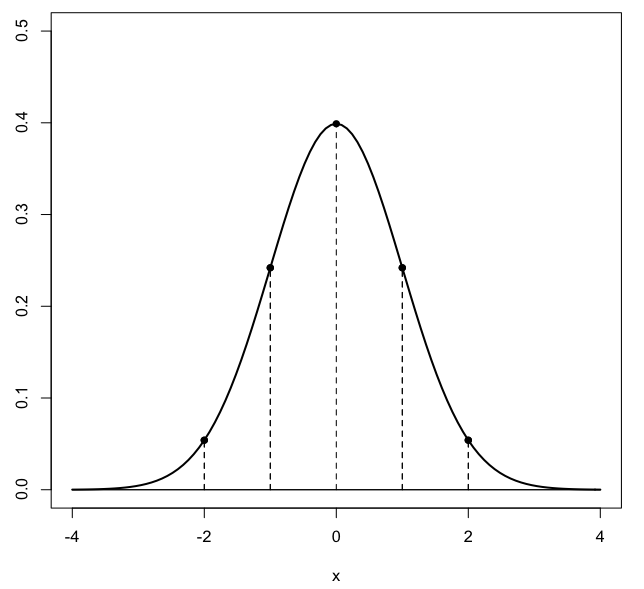
\includegraphics [scale=0.4] {gauss3.png} \end{center}

%break
\title{Eigenvalues and eigenvectors}
\date{}

\begin{document}
\maketitle
\Large


An eigenvector of a square matrix is a non-zero vector that, when multiplied by the matrix, yields a vector that is parallel to the original.  That is
\[ A\mathbf{v} = \lambda \mathbf{v} \]
The result of the matrix $A$ multiplying its eigenvector $\mathbf{v}$, $A \mathbf{v}$, gives a vector that is unchanged except for a multiplicative constant, $\lambda$, called the eigenvalue.  The prefix "eigen" is related to the German for "self".

As a simple example, consider the matrix for reflection across the axis $y=x$.  This matrix just switches $x$ for $y$.  Call it $R$:
\[
R = 
\begin{bmatrix}
0 & 1  \\  
1 & 0  
\end{bmatrix}
\]
Most vectors end up pointing in a different direction after reflection across the axis.  Which ones don't?  Any vector that is a multiple of $\mathbf{v}= \ <1,1> $, will end up exactly the same, since $\mathbf{v}$ lies exactly along $y=x$.  So we expect that $\mathbf{v}=\ <1,1>$ is an eigenvector of $R$ and that the eigenvalue $\lambda$ will be equal to $1$.

Solving such a problem formally, finding the eigenvectors and eigenvalues for a matrix, starts by rearranging what we had above and solving
\[ A\mathbf{v} - \lambda \mathbf{v} = 0 = (A-\lambda I)\mathbf{v} \]
A standard result from early linear algebra is that this equation has non-zero solutions $\iff det((A-\lambda I) = 0$).

So we set up the subtraction
\[
A-\lambda I = 
\begin{bmatrix}
-\lambda & 1  \\  
1 & -\lambda  
\end{bmatrix}
\]
The equation of the determinant is 
\[ \lambda^2 - 1 = 0  \]
The solutions are $\lambda = -1,1$.  How to find the eigenvector corresponding to a particular eigenvalue?  We write out the matrix multiplication with $\mathbf{v} = \ <x,y>$
\[ 0x + y = \lambda x \]
\[ x + 0y = \lambda y \]
For $\lambda=1$ we need 
\[ A \mathbf{v} = \mathbf{v}  \]
\[ 0x + y = x \]
\[ x + 0y = y \]
Clearly $x=y$, so this eigenvector is as we predicted.  However, there is a second eigenvalue ($\lambda = -1$).  What's up with that?
\[ A \mathbf{v} = -\mathbf{v}  \]
\[ 0x + y = -x \]
\[ x + 0y = -y \]
Now we have $x=-y$, the eigenvector for $\lambda=-1$.  And we see it!  A vector that is \emph{perpendicular} to the axis of reflection goes right straight through, it appears reflected on the other side with identical length, but multiplied by $-1$.

Some well-known matrices don't have real eigenvalues.  Consider the matrix for $90^\circ$ rotation counter-clockwise
\[
R_{90}  = 
\begin{bmatrix}
0 & -1  \\  
1 & 0  
\end{bmatrix}
\]
We end up with the equation to solve
\[ \lambda^2 + 1 = 0  \]
This simple equation has no real solutions (just $i$ and $-i$).  And if you think about it, what kind of vector would be unchanged by a $90^\circ$ rotation?

What about 
\[
R_{180} = R_{90} \times R_{90}  =
\begin{bmatrix}
0 & -1  \\  
1 & 0  
\end{bmatrix}
\begin{bmatrix}
0 & -1  \\  
1 & 0  
\end{bmatrix}
=
\begin{bmatrix}
-1 & 0  \\  
0 & -1  
\end{bmatrix}
\]
If we rotate any vector $\mathbf{v}$ by $180^\circ$, it is the same as multiplying by $-1$.  So we expect every vector to be an eigenvector with eigenvalue $\lambda = -1$.  The equation for the determinant is
\[ (-1 - \lambda)^2 = 0 \]
\[ (-\lambda - 1)^2 = (-1)^2(\lambda + 1)^2 = (\lambda + 1)^2 \]
So the two eigenvalues are both $\lambda = -1$, and the \emph{eigenspace} is every vector.
\[
\begin{bmatrix}
-1 & 0  \\  
0 & -1  
\end{bmatrix}
\begin{bmatrix}
x  \\  
y  
\end{bmatrix}
=
\begin{bmatrix}
-x  \\  
-y  
\end{bmatrix}
\]


As another example, consider this matrix
\[
T = 
\begin{bmatrix}
2 & 1  \\  
1 & 2  
\end{bmatrix}
\]
Multiplying by $T$ turns $\mathbf{v} = <1,1>$ into $<3,3>$ so it looks like $\mathbf{v}$ is an eigenvector of the matrix, with eigenvalue $3$.  This transformation stretches vectors, but also changes the orientation for most.  The ones that don't change orientation are $\mathbf{v} = <1,1>$ and $\mathbf{w} = <-1,1>$  Let's solve it.  We need
\[
\begin{vmatrix}
2-\lambda & 1  \\  
1 & 2-\lambda  
\end{vmatrix}
= 0
\]
We have the $\emph{characteristic equation}$
\[ (2-\lambda)^2 - 1 = 0 \]
\[ \lambda^2 - 4\lambda +3 = 0 \]
\[ (\lambda - 3) ( \lambda - 1) = 0 \]

The roots are $\lambda = 3, 1$.  We already found the eigenvector for $\lambda=3$.  Now for the other, we have
\[
\begin{bmatrix}
2 & 1  \\  
1 & 2  
\end{bmatrix}
\mathbf{w}
= \mathbf{w}
\]
\[ 2x + y = x \]
\[ x + 2y = y \]
The solution is $\mathbf{w} = \ <1,-1>$ (again).  A vector perpendicular to $\mathbf{v}$ is also not turned by this matrix.  And it's not stretched either.
\vspace{5 mm}

See the animation:
\url{http://en.wikipedia.org/wiki/Eigenvalues}
\vspace{5 mm}

Most vectors can be decomposed into two pieces that are parallel and perpendicular to $\mathbf{v} = \ <1,1>$.  The part that is parallel will be stretched by a factor of 3.  We predict that $<1,1> + <-1,1> \ = \ <0,2>$ will become $<3,3> + <-1,1> \ = \ <2,4>$.
\[
\begin{bmatrix}
2 & 1  \\  
1 & 2  
\end{bmatrix}
\begin{bmatrix}
0  \\  
2  
\end{bmatrix}
=
\begin{bmatrix}
2  \\  
4  
\end{bmatrix}
\]
Looks good to me.

Finally, consider a permutation matrix in R3, for example

\[
\begin{bmatrix}
0 & 1 & 0  \\  
0 & 0 & 1  \\  
1 & 0 & 0 
\end{bmatrix}
\]

\[
P -\lambda I = 
\begin{bmatrix}
-\lambda & 1 & 0  \\  
0 & -\lambda & 1  \\  
1 & 0 & -\lambda 
\end{bmatrix}
\]

The determinant is set equal to zero

\[ -\lambda(\lambda^2) + 1 = 0 \]
\[ 1 - \lambda^3 = 0 \]
\[ \lambda^3 = 1 \]

This has one real root ($\lambda = 1$), and two complex roots which we obtain by recalling that

\[ a^3 - b^3 = (a-b)(a^2 + ab + b^2) \]
\[ \lambda^3 - 1^3 = (\lambda-1)(\lambda^2 + \lambda + 1) \]

The first term is our real root.  The complex roots come from the quadratic equation for the second term:

\[ \frac{-1 \pm \sqrt{1 - 4}}{2}  \]

Hence, 
\[ \lambda_1 = 1 \]
\[ \lambda_2 = -\frac{1}{2} + i\frac{\sqrt{3}}{2} \]
\[ \lambda_3 = -\frac{1}{2} - i\frac{\sqrt{3}}{2} \]

Notice that the two complex roots are complex conjugates.  

Now, for the real eigenvalue $\lambda_1 = 1$, we need to an find eigenvector

\[
\begin{bmatrix}
0 & 1 & 0  \\  
0 & 0 & 1  \\  
1 & 0 & 0 
\end{bmatrix}
\begin{bmatrix}
x  \\  
y  \\  
z 
\end{bmatrix}
=
\begin{bmatrix}
x  \\  
y  \\  
z 
\end{bmatrix}
\]

From these equations, $y = x, z = y$, and $x = z$.  It looks like $\mathbf{v} = \langle 1,1,1 \rangle$ will do.

\subsection*{trace and determinant}

One last thing, the trace is the sum of the diagonal entries on a matrix.  The trace is also equal to the sum of the eigenvalues.  And the determinant of the matrix is the product of the eigenvalues.
\[ trace = \sum \text{eigenvalues} \]
\[ det = \prod \text{eigenvalues} \]
Let's just check this for the matrices used as examples here
\[
A = 
\begin{bmatrix}
0 & 1  \\  
1 & 0  
\end{bmatrix},
\ \ \lambda = \pm 1
\]
They add to give 0 and multiply to give -1.  $\checkmark$
\[
R_{90}  = 
\begin{bmatrix}
0 & -1  \\  
1 & 0  
\end{bmatrix}, 
\ \ \lambda = \pm i
\]
They add to give 0 and multiply to give 1.  $\checkmark$
\[
R_{180} = 
\begin{bmatrix}
-1 & 0  \\  
0 & -1  
\end{bmatrix}, 
\ \ \lambda = -1,-1
\]
They add to give -2 and multiply to give 1.  $\checkmark$
\[
\begin{bmatrix}
2 & 1  \\  
1 & 2  
\end{bmatrix}
\ \ \lambda = 1,3
\]
They add to give 4 and multiply to give 3.  $\checkmark$

For the very last example we had

\[ \lambda_1 = 1 \]
\[ \lambda_2 = -\frac{1}{2} + i\frac{\sqrt{3}}{2} \]
\[ \lambda_3 = -\frac{1}{2} - i\frac{\sqrt{3}}{2} \]

If the trace (which is real) is the sum of the eigenvalues, that explains why the two complex eigenvalues must be conjugates.

Here we have that the sum of the eigenvalues is equal to $1 - 1/2 + z - 1/2 - z = 0$, which is also the trace.

\end{document}  